\documentclass[english,a4paper]{article}
\usepackage[T1]{fontenc}
\usepackage[latin9]{inputenc}
\usepackage{graphicx}
\usepackage{babel}
\usepackage{listings}
\usepackage{verbatimbox}
\renewcommand{\lstlistingname}{Listing}

\begin{document}

\title{A JIT-Less Type-Mapped Dynamic-ISA Virtual Machine for Many-Instance
Applications}

\maketitle
\rule[0.5ex]{1\columnwidth}{2pt}

\begin{figure}[tph]

 \centerline{ 
\includegraphics[scale=0.5]{nmmu.jpg}}
\end{figure}

\author{ \centerline{ Author: Douglas Bentley}}
\author{ \centerline{ Supervisor: Kevin Naud�}}

\rule[0.5ex]{1\columnwidth}{2pt}

\title{Submitted in partial fulfilment of the degree Baccalaureus Scientiae
(Honores) in Computer Science at the Nelson Mandela Metropolitan University}

\newpage{}

\section*{Acknowledgements}

\newpage{}

\section*{Abstract}

\newpage{}

\section*{Declaration of Own Work}

\newpage{}

\section*{List of Figures}

\newpage{}

\section*{List of Tables}

\newpage{}

\section*{Table of Contents}

\newpage{}

\section{Introduction}
In the last x years, software applications programming has seen a shift away from compiled languages that run natively on hardware towards interpreted languages that require the use of another program, called an interpreter to execute them. This has several advantages. One is portability. If you have an interpreter that runs on different hardware and operating systems you can run your interpreted programs in these different environments with no change to your code. Another advantage is that memory can be managed. This helps prevent bugs and security issues and takes the burden of managing memory off the programmer. The disadvantage of interpreted languages is that they must necessarily be slower than equivalent native code. For systems programming and big-budget video games, natively compiled languages are preferred as the performance hit is considered to be too great but for general applications programming interpreted languages are preferred. For business systems this usually means Java and C\# and for web development this means JavaScript and PHP.

Given the popularity of these languages, research into interpreter performance is important. 

\subsection{Dynamically Typed Languages}
Dynamically typed languages are the foundation on which the modern website is built. Currently there are two major web-development languages: JavaScript and PHP. All major browsers have JavaScript engines (virtual machines) which can interpret and execute JavaScript code. Developers use JavaScript to create interactive websites. PHP on the other hand is the most commonly used language for server-side scripting. This is what allows web pages to have dynamic content. Pages can be generated as needed and personalised for each user using PHP. Several other dynamically typed languages are commonly used for server-side scripting. These include Ruby (Ruby on Rails), Python (Django) and JavaScript (Node.js).

Dynamically typed languages also play the role of "glue" languages that stick together different software components. A prime example is the Lua programming language which is used for video game scripting. In this instance the video game's engine is written in C++ for better performance but the logic of the game is a Lua script that runs on the Lua virtual machine. Since Lua is a higher-level language it can be used to more easily express the less performance-critical elements of the game. Another example is the Bash command language which acts as glue for the GNU core utilities which are written in C. Each program in the coreutils performs a simple operation but these can easily be composed using a Bash script or command to create complex behaviour. Dynamic languages are ideal for tasks like this because they have simple, terse syntax and powerful abstractions.

\subsection{Interpreting Dynamically Typed Languages}
Dynamically typed languages are commonly paired with an interpreter. That is, these languages are not compiled to machine code that can be run on some architecture. Instead, it is the job of a seperate program to determine the meaning of the program and perform the instructions on actual hardware. There are three main approeaches to interpreting dynamically typed languages:

\subsubsection{Line by Line}
In line by line interpretation the program is parsed one line at a time. Each line is executed before moving on to the next line in the program. This is ideal for command-line interface operating systems where the primary mode of interaction is entering single-line commands. Some examples of langauges with this type of interpreter are: Bash, CMD.EXE, Python and Ruby.

\subsubsection{Abstract Syntax Tree}
Abstract syntax tree or AST interpreters parse the entire program and build an abstract syntax tree that represents the structure of the program. This tree can then be traversed in the correct order to execute the program. Exmaples??

\subsubsection{Bytecode}
Bytecode interpreters interpret a pre-compiled bytecode that is much like machine code executed by the CPU. This can be stored compactly and executed by decoding the opcode and performing the instruction associated with it. This approach is found in the statically typed languages Java and C\# but dynamically typed languages like Lua share the same approach. Bytecode interpreters are also called virtual machines because of they perform the same tasks as a real CPU: fetching, decoding and executing instructions.

\subsection{Workings of a Virtual Machine} 
When reading in bytecode, the virtual machine needs some whay to know what it is currently reading. This is slightly more complex than just keeping track of how far into the program the VM has read as the program can have instructions that allow the virtual machine to jump between different points in the program. This is how loops and functions are implemented. The instruction pointer (or IP) is used for this purpose.
 
The core of the virtual machine is its dispatch mechanism. The machine reads the instruction that the instruction pointer points to and then must determine what subroutine needs to be called to execute the instruction. Selecting and moving execution to this subroutine is called ``dispatch''. How to implement this dispatch mechanism is a complex topic that will be discussed in more depth in chapter 3.

The subroutines are the virtual machine's instruction set. A VM usually has instructions for performing arithmetic instructions (add and divide), bit manipulation (xor or and), controlling the flow of the program (jump and various conditional jumps) and for storing and accessing values. The design of an instruction set, much like a CPU's instruction set is a creative process. The set of instructions a virtual machine has is the decision of the designer.

\subsection{Project Objectives}
The objective of this project is to implement and benchmark a novel virtual machine design for a dynamically typed language. In order to benchmark the performance of the virtual machine an additional virtual machine must be developed using a more conventional VM design against which the benchmark running times can be measured. The project will determine what kind of performance benefits can be gained from this type of virtual machine.

\subsection{Project Scope}

The project is to develop an implementation of a VM of this nature and run predetermined benchmarks on it against an alternate version of it that does not make use of type-mapping. This experiment should show what benefits the approach has. There will be no compiler or assembler implementation required and the VM will not be required to perform garbage collection. The VM will also not have to be robust in how it interacts with the operating system it is running on nor in how it handles errors.

\subsection{Risks}

The risks of the project are mainly about its structure and how it can be criticised. The VM will be running predefined benchmarks. If it performs those well at the expense of its general usefulness the project can be criticised. All of these sorts of criticisms can be mitigated so long as the goal of the project is kept in mind at all times. Learning as much as possible about how well the idea works should always take precedence over trying to make results look good. Whether the VM performs better or not is important knowledge and being as careful as possible about discovering that accurately is extremely
important.

\subsection{Overview of Treatise}

In chapter 2, the virtual machine as a concept will be introduced and the different types of virtual machines will be covered. Existing solutions to the problem of a VM for dynamically typed language will be examined and some theory about modern processors will be covered. This theory informs some of the design decisions of the virtual machine.

In chapter 3, the implementation details and decisions made in the design of the VM will be covered. This chapter will cover how the VM works, what instructions it supports and how it implements these instructions. This chapter will also discuss the trade-offs of the virtual machine's design against the conventional approach.

In chapter 4, the experimental design and benchmarks will be discussed. Which benchmarks were chosen and what they can tell us about the virtual machine will be discussed in this chapter. It will also detail the exact details of how the experiment was conducted so that it may be repeatable with similar hardware.

In chapter 5, the results of the experiment will be discussed and analysed and the performance benefits of the virtual machine will be examined.

Lastly in chapter 6, conclusions will be drawn about whether and in what instances the implementation for the virtual machine is useful and what its strengths and weaknesses are.


To be completed
\newpage{}

\section{Literature Review, Existing systems and Modern Processors}

\subsection{Virtual Machines}

To best describe the virtual machine presented in this treatise, a quick summary of virtual machines follows. The heirarchy of virtual machines is presented and our virtual machine is situated within it. Some important virtual machine terminology is introduced. 
A \emph{virtual machine} or \emph{VM} is a computer program that ``executes software in the same manner as the machine for which the software was developed'' \cite[pg9]{JamesE.Smith2005}. This program is designed to run on some real machine. We call the real machine that a virtual machine is running on the \emph{host} and the virtual machine the \emph{guest. }The guest machine provides an execution environment for software that is designed to run either on the guest itself or on an actual machine that the virtual machine is emulating. This means that we can use a virtual machine to run programs that are incompatable with the host. The virtual machine allows this by providing a mapping of its state to the state of the host machine on which it is running \cite[pg4]{JamesE.Smith2005}.

\subsection{The Types of Virtual Machines}

Virtual machines come in two varieties: \emph{process }virtual machines and \emph{system} virtual machines.

A process virtual machine is ``capable of supporting an individual process''\cite[pg9]{JamesE.Smith2005}. This means that the host runs the guest for as long as a process on the guest machine needs it. Once the process has completed its execution the guest machine terminates\cite[pg9]{JamesE.Smith2005}. An example of a process virtual machine is the Java Virtual Machine or JVM. All java programs run on the JVM. An instance of the JVM is started when you execute a java program and killed when its execution is complete.

A system virtual machine ``provides a complete system environment'' ''\cite[pg9]{JamesE.Smith2005}. This means that it can support an entire operating system on the guest machine and the many processes that the guest operating system executes. A system virtual machine will terminate when the system is shut down.

\subsection{The Types of Process Virtual Machines}

Since this treatise outlines a process virtual machine we shall look at the different types of process virtual machines and ignore the finer details of system virtual machines. Process virtual machines can be divided into two categories: \emph{multiprogrammed} \emph{systems} and \emph{dynamic} \emph{translators}. These are divided along whether or not the guest machine uses the same instruction set architecture as the host machine.

With multiprogramming the guest and host use the same instruction set. Multiprogramming is supported by most operating systems and allows a user to run many processes at once by making each process think it has access to an entire machine instead of only part of a machine ''\cite[pg13]{JamesE.Smith2005}. The OS creates an environment per process that it terminates when that process ends execution.

With dynamic translators the instruction set of the host and guest generally do not match. The virtual machine translates blocks of instructions meant for the machine it is emulating and translates them into instructions to be run on the host. Not all code is translated in a dynamic translater. Only code that is used often enough will be translated as there is an overhead involved with translating code. The code that is not translated is interpreted. Interpreted instructions are read, their meaning interpreted and then executed. This interpretation step must happen each time a piece of code is executed so code that is executed enough times will be dynamically translated and cached so later execution is faster. Dynamically translating in this manner is known as ju\emph{st-in-time compilation} (JIT compilation).

\subsection{Dynamic vs Statically Typed Programming Languages}

A dynamically typed language is one in which the type information is associated with values \cite[pg4]{RobertoIerusalimschy}(REF lua VM intro). An example of a dynamically typed language is javascript where the var keyword is used for variables and the type is inferred from the value stored into a variable. A statically typed language is one in which the type information is associated with the variable. An example of this is java where variables are declared using keywords that define their type (\emph{int}, \emph{string} etc).

\subsection{Where Our VM is Situated}

The virtual machine described in this treatise is a process virtual machine. This process machine will have a new instruction set architecture and hence will differ from any host machine's ISA. The virtual machine does not make use of JIT compilation. It is entirely interpreted. It is also dynamically typed.

\subsection{A Virtual Machine for Many Instance Applications}

Modern process virtual machines make use of JIT compilers. Both JVM and .Net make use of a JIT compiler \cite{MSDN,Oracle}. For applications that run many concurrent instances, like a web server which which starts up a new process for every client, a virtual machine that makes use of a JIT compiler defeats the benefits of read-only memory sharing. Since memory sharing is not possible when using a JIT compiler, if we wish to take advantage of it a JIT-less virtual machine is needed. However the JIT compiler compiler is an important feature of a VM that allows for code given to it at runtime to be compiled into machine code that can run directly on the host. This compiled code is cached and allows for future execution to be faster. Sacrificing the JIT compiler to allow memory sharing presents us with a need to find alternative ways to let our programs execute quickly.

\subsection{Type-Mapping and Argument Case Expansion}

A type-mapped VM is one which keeps track of the state of the types of its registers. This is beneficial because every instruction in a conventional VM design must first verify the types of its inputs before it can act on them. These type checks can be eliminated with type-mapping and intructions can be customised based on the types of the inputs they receive. This is closely coupled with the idea of argument case expansion. For Type-Mapping to be effective the VM must dispatch on its current type state. This is what eliminates the type checking step. But if the VM does not also dispatch on the arguments for the next instruction it cannot know which version of the instruction is appropriate. Argument case expansion means having a version of each instruction for every combination of arguments.

\subsection{Modern Processor Architecture}

In order to create an efficient VM, we need first understand how modern processors work and what some of the bottlenecks for our VM's execution might be. For example, \emph{threading techniques} (not to be confused with threads in application programming) are commonly used in VM design. These take advantage of a feature of modern processors called the \emph{Branch Target Buffer} or BTB. The BTB exists to aid a process called \emph{branch prediction}. Branch prediction itself can only be explained once we know about how modern processors make use of \emph{pipelining} to increase their throughput. As you can see, an understanding of modern computer architectures is needed before we can begin a discussion of VM design.

\subsubsection{Pipelining}

Pipelining is a process in which a processor's instruction processing cycle is shared by many consecutive instructions at once. The instruction processing procedure is split up into smaller stages that can execute simultaneously. An example of this is the classic RISC pipeline{[}x{]} which to divides instruction processing into the following steps: Instruction Fetch (IF), Decode (ID), Execute(EX), Memory Access (MEM) and Writeback (WB). Each instruction passes a stage and leaves that part of the processor free to perform that stage on the next instruction. Thus many instructions (as many as there are stages) can be processed at once, instead of each instruction having to be completely processed before the processor is free to move onto the next instruction. The process is analogous to an asssembly line, where many cars can be assembled at the same time, each in a different stage of assembly.

\begin{figure}[tph]
\protect\caption{\protect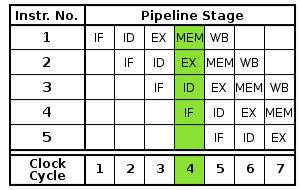
\includegraphics[scale=0.5]{pipeline}}
\end{figure}

In \emph{fig1} we see that the first instruction as currently performing memory access while the second EXecutes and the third is being Decoded. Up to 5 instructions can be processed simultaneously.

When pipelining an interesting situation occurs in the case of flow control instructions. These are instructions that cause execution to move to some other point in the program. The point at which we know which instruction comes next (called \emph{branch resolution}) is usually later in the pipeline. Thus the processor cannot queue up the next instruction as it does not know which instruction will execute next. Branch prediction is used in modern processors to try to keep the pipeline as full as possible and not waste time waiting
for this information to be known.

\subsubsection{Branch Prediction}

Instead of filling up the pipeline with no operation instructions until we know where to branch, with branch prediction we guess which branch will be taken and place the instructions from the predicted branch into the pipeline. When we know where the branch operation should have taken execution we either throw out our newly pipelined instructions (this is called \emph{pipeline flushing}) if the prediction was incorrect or continue execution if it was correct. The more stages the pipeline has before branch resolution, the more of a performance benefit correct predictions become for programs with many control flow instructions. A Virtual Machine is such a program. This is because a VM must branch to the correct code for each instruction it executes. Writing code that allows for increased branch prediction accuracy is thus very important for VM efficiency.

Predicting a branch means we must predict if that branch is taken or not and what the target of that branch is if it is taken. Modern processors have a Branch Target Buffer where the target adresses of previously taken branches are cached. So upon arrival at a branch that has been previously taken, we guess if it will be taken and if it is we begin speculatively executing from the address stored in the BTB.

\subsubsection{Cache}

Modern processors make use of different levels of cache to allow for faster memory access. Ideally we would like to have an infinite amount of memory with no time cost for accessing it. The reality is that the larger memory is, the slower it becomes to access it {[}???{]}. In order to get closer to the ideal modern processors make use of cache. It takes around 100 cycles for Intel's Intel i7-4770 (Haswell) architecture to access memory. Cache allows us get get closer to the ideal case by keeping commonly accessed memory closer to the CPU in levels of increasingly smaller, faster and more expensive (to manufacture) memory. The Haswell has 32KB of L1 data cache and 32KB of L1 code cache. These are located on the CPU itself {[}x{]} and can be accessed in around 4 cycles{[}x{]}. It also has 256KB of L2 cache and 8 MB of L3 cache. Caching works on the principal of locality of access. If you access memory in more or less the same area a lot, that acess is much faster than if you hop around from place to place. We should try to take advantage of cache in our VM's design.

\subsection{Traditional Implementation of High Level VMs}

\subsubsection{Dispatch and Threading}

Dispatch is the process of fetching, decoding and starting the next instruction to be run by a virtual machine {[}x{]}.

The simplest way to implement a virtual machine is to make use of a switch statement in a loop. This is called switch dispatch. Here is a simplified version to illustrate:

\begin{lstlisting}
typedef enum { add /* ... */ } Inst; 

void engine() 
{ 
	static Inst program[] = { add /* ... */ }; 
	Inst *ip = program; 
	int *sp; 

	for (;;) 
		switch (*ip++) 
		{ 
		case add: 
			sp[1]=sp[0]+sp[1]; 
			sp++; 
		break; 
		/* ... */ 
	}
} 
\end{lstlisting}

This approach is problematic because the switch statement means that there is only ever a single entry in the Branch Target Buffer used for dispatch . This means that the number of mispredictions will be large as the target of the branch will change for each new instruction we branch to. This problem may even be magnified by the fact that this specific VM implementation has far more instructions than usual as it requires several specialised versions of every instruction.

A faster alternative to switch dispatch is direct threading\cite{Ertl}. The name threading comes from the idea of the execution threading its way from one instruction to the next {[}x{]}. In direct threading the program is stored as a list of addresses of instructions and the code for each instruction includes a dispatch portion which jumps to the address of the next instruction to be executed.

\begin{lstlisting}
typedef void *Inst; 

void engine() 
{ 
	static Inst program[] = { &&add /* ... */ }; 
	Inst *ip = program; 
	int *sp; 
	
	goto *ip++; /* dispatch first VM inst. */ 

add: 
	sp[1]=sp[0]+sp[1]; 
	sp++; 
	goto *ip++; /* dispatch next VM inst. */ 

}
\end{lstlisting}

Another method is indirect threading. In indirect threading we keep a lookup table of the addresses of code for each instruction and have each instruction jump to the next by reading the opcode of the next instruction from the program, looking up the address of the code for that instruction in the table and then jumping to that instruction.

\begin{lstlisting}
typedef void *Inst; 

void engine() 
{ 
	static Inst lookup[] = { &&add, &&sub /*...*/ }
	static int program[] = { 0, /* ... */ }; 
	int *ip = program; 
	int *sp; 
	
	goto *ip++; /* dispatch first VM inst. */ 

add: 
	sp[1]=sp[0]+sp[1]; 
	sp++; 
	goto lookup[*ip++]; /* dispatch next VM inst. */ 
}
\end{lstlisting}

Direct and inderect threading make much better use of the branch target buffer. Instead of a single entry in the BTB, with direct threading we have an entry per instruction, so instructions that commonly follow each other have a better chance of being predicted.

All code in this section is from or adapted from \cite{M.AntonErtl2003}.


\subsubsection{Registers VS Stacks}


In a stack virtual machine, instructions act on members of the stack. Arguments and return values for instructions are often implicit and thus instructions can be smaller. For instance a stack implementation of a = b + c would first push b and c onto the stack, then call the add instruction which has no arguments. Add pops b and c off the stack and pushes b+c back onto the stack. This value is then popped off the stack and stored.


For a register machine, a similar piece of code would have values for b and c in registers and an add instruction is called with a, b and c as arguments. This instruction would compute b+c and store it in a regsiter.

Widely used process virtual machines make use of a stack architecture. Both the Java Virtual Machine (JVM) and Microsoft's Common Language Runtime (CLR) make use of stack virtual machines{[}x{]}. 

\subsubsection{JIT Compilation}

Both the JVM and CLR make use of JIT compilation {[}x{]}. JIT compilation allows for code that is executed often enough to be compiled into native machine code at runtime. JIT compilation does not preclude the bytecode of a many-instance application being shared but each instance of the application is JIT compiling that code. So it is likely that the same bytecode is being compiled in many different processes at the same time.

\subsection{VM Interpreter Reseach}

James R. Bell introduced the concept of threaded code in 1973. The Fortran IV compiler was written to generate threaded code.\cite{Bell}  Yuhne Shi\cite{Shi2007} found that a well-implemented register VM is a more efficient option when speed of execution is more important than the size of the code to be executed.

Ertl and Gregg found that in their benchmarks 3.2\%\textendash 13\% of all executed instructions were indirect branches and that switch dispatch on an architecture with a BRB resulted in 81\%-98\% branch prediction misses \cite{M.AntonErtl2003}. They also found that direct threading resulted in 50\%-63\% branch prediction misses.

\subsection{Our Implementation}

\subsubsection{Virtual Machine Design Details}

The virtual machine described in this treatise is a register machine. It has 6 general purpose registers and 3 special purpose registers. The VM is for a dynamically typed language. Each register stores 'values' and all instructions act on those values. The type of a value is stored together with the data for that value. These are implemented in C as tagged unions. The VM has only two types: integer and pointer. 

The 3 special purpose registers are:
\begin{enumerate}
\item The program counter (pc), which keeps track of where we are in the
program
\item The frame pointer (fp), which points to the bottom of the latest stack
frame
\item The type state (ts), which keeps track of the current state of types
in the registers
\end{enumerate}

\subsubsection{Type-Mapping}

The virtual machine does not make use of the usual opcode and arguments arrangment used in register machine interpreters. Usually, the interpreter reads in some instruction stored as an opcode and the arguments for that opcode at the same time. In \emph{fig 2} we see a 16 bit instruction composed of a 4 bit opcode in the high bits, followed by two 6 bit operands or aguments. The interpreter performs the necessary shifts and bitmasking to get the values out of the fields.

\begin{figure}[tph]
% \protect\caption{\protect\includegraphics[scale=0.6]{/home/stevetest/opcode}}
\end{figure}

In our VM instructions for programs are stored as opcodes only with no arguments. That is because we have a version of each instruction for every combination of registers as inputs. Because we have 6 registers and a maximum of two arguments per instruction that means that we can have a maximum of 6\textasciicircum{}2 versions of each instruction. This saves us the process of extracting arguments at the expense having to have more versions of the instruction{[}why are we doing it this way actually?{]}. The opcode implicitly stores the argument information.

The opcode is not the only information the VM uses to select code, however. The \emph{ts} register keeps a record of the type of every register. It is a 6 bit number where each bit tells us the current type of a register. Thus for every opcode, there are 2\textasciicircum{}6 different states the VM could be in. With this information we know the arguments and types and can jump to specialised code that acts on arguments of those types. A good way to think about it is to imagine it as a 2D lookup table (even though the implementation is 1D). On the y-axis we have the opcodes for all the versions of the instructions and on the x-axis we have the current state from 0 to 63. At the intersection of these we store the address of the code we jump to for that instruction.

Now since we only have integers and pointers it may, at first glace, seem pointless to have specialised instructions since most of the time using pointers in an instruction meant for integers is illegal. However this method elliminates the type checking involved in instructions for a dynamic-ISA VM. Normally for each instruction we would have to check the validity of the arguments first before we can perform the instruction, but with this method we already know the types and so we can just jump directly to code for those types or an error if the arguments are illegal.

\subsubsection{Indirect Threading}

This VM will make use of indirect threading. Though indirect threading is slower than direct threading {[}x{]} because it must first complete the lookup step before it can branch to the next instruction, the program code used by the VM is intended to be shared by many instances of the VM. This cannot be achieved with direct threading as the addresses of each instruction in each instance may be different{[}x{]}. Also because our dispatch is based on the runtime state of the virtual machine (the st register) even if addresses were the same between instnces we can't represent code in terms of those addresses as we don't know the state information until runtime so we can't choose which address should be used to replace the opcode. With Indirect threading's lookup table we can share the code in its opcode form and perform the correct jumps for each instance of the VM by consulting the state register and looking up the addresses in the lookup table.

\section{Solution Design}

Three virtual machines are presented as solutions. These VMs are spaced along a scale for how much they expand out the behaviour of each instruction to match the state of the virtual machine. At the lowest end of the scale is the control virtual machine which shall be referred to as the Conventional VM. One step up from that is a VM that expands out all cases of arguments for each instruction. This will be referred to as the Hybrid VM. A further step takes us to the Type-State virtual machine which, like the hybrid VM, expands out all cases of arguments for each instruction, but then further expands out for every case of the combinations of types those arguments could take on.

On the lowest end of this scale the VM is simpler to implement and uses fewer instructions, but each instruction is less specific and so the complexity lies within the instructions. This is the conventional design for this type of VM.

On the highest end of the scale the VM is more difficult to implement and uses more instructions, but each instruction is very specifically geared to exact state of the VM so each instruction is very simple.

\subsection{Common Elements}

The three virtual machines are designed to be as similar as possible except for the aspects that the experiment examines. Those elements common to all VMs shall be expanded upon here and those specific to each shall be examined seperately.

\subsubsection{Values}


\begin{lstlisting}
typedef struct ValueStruct value;
struct ValueStruct
{
	int tag;
	union
	{
		int64_t i;
		void *p;    
	};
};
\end{lstlisting}

As this is a dynamic ISA virtual machine, types are associated with values instead of variables [lua VM]. The implementation for a value is simple enough to include here.

A

\subsubsection{Objects}

Objects are a simple built-in data structure for storing ordered fields of values. Objects are implemented as a struct with an array of values and an integer field for storing the length of the array. This integer field is also
used to store 

\subsubsection{Buffers}

Buffers are a data structure that exposes the native byte to the VM so that string handling may be performed without having to create a value for each character. The implementation is, once again a struct with an array of bytes and a size field that holds the length of the array.

\subsubsection{Registers}

All virtual machines make use of 6 general purpose registers. These registers are implemented as an array of 6 values. A further two registers are found in all VMs, that is the program counter, which will be referred to as PC and the frame pointer which will be referred to as FP. These are a 64 bit integer and a value pointer respectively.

\subsubsection{Stack Frames}

All VMs make use of identical Stack Frames for subroutine calls. Each stack frame stores: 

\begin{itemize} 
	\item The previous FP, PC and an additional register that goes unused except in the Type-State VM. 
	\item The general purpose registers except the first and last
	\item The local variables used in that stack frame 
\end{itemize}

Registers are saved upon calling a subroutine and restored when the subroutine returns. The first and last general purpose registers are used for return values.

\subsubsection{Addressing}

\subsubsection{Instructions}

All virtual machines support an identical set of instructions. How these are implemented is quite different for each VM but the functionality of each instruction does not change between virtual machines. 

Instruction words are 16 bits long.	Each instruction may have a maximum of two operands. If the instruction has multiple operands and a result, the result will be stored in the first of the two operands.

Instruction operands refer to one of the 6 general purpose registers. In some cases the next instruction word is a 16 bit constant value that is used by the instruction and in others the next instruction word is used as a 16 bit PC-relative address for a 64 bit constant value. These will be denoted as const16 and const64 respectively and their implementation will be expanded upon later.

In some cases, specific argument combinations for an instruction have been removed as they produce trivial results. For instance the subtract operation cannot be used with the same register for both arguments. Since the result of this operation is always zero and there already is an instruction to set a register to zero, there is no need to include this case. This has little bearing on the conventional VM (which can do these operations) but plays a role in the other two VMs. 

The set of instructions is as follows:

\subsection*{Arithmetic Instructions}

Arithmetic instructions provide some basic arithmetic operations for registers that contain integers. If a register that does not contain an integer is selected, an error is signalled and the VM halts. All arithmetic instructions increment the program counter. Those that make use of a constant that is looked up in the next instruction word increment the program counter again so that the PC points to the next instruction and not the data contained in the next word. The PC is incremented after the operation performed by the instruction.

\addvbuffer[12pt 8pt]{\begin{tabular}{| l | l |}
		\hline
		$add(g _{i}, g _{j}) $ & $ g _{i} \longleftarrow  g _{i} + g _{j} $\\
		\hline
		$addc(g _{i}, const _{64}) $ & $ g _{i} \longleftarrow  g _{i} + const _{64} $\\
		\hline
		$sub(g _{i}, g _{j\neq i}) $ & $ g _{i} \longleftarrow  g _{i} - g _{j} $\\
		\hline
		$csub(const _{64}, g _{i}) $ & $ g _{i} \longleftarrow const _{64} - g _{i} $\\
		\hline
		$mul(g _{i}, g _{j}) $ & $ g _{i} \longleftarrow  g _{i} \times g _{j} $\\
		\hline
		$mulc(g _{i}, const _{64}) $ & $ g _{i} \longleftarrow  g _{i} \times const _{64} $\\
		\hline
	
		$div(g _{i}, g _{j\neq i}) $ & 
		\begin{tabular}{@{}l@{}}
			$ g _{i} \longleftarrow  g _{i} \div g _{j}$ \\		
			$g _{0} \longleftarrow  g _{i} \textbf{ mod } g _{j} $\end{tabular}\\
				 
		\hline
		$div(g _{i}, const _{64}) $ & 
		\begin{tabular}{@{}l@{}}
			$ g _{i} \longleftarrow  g _{i} \div const_{64}$ \\		
			$g _{0} \longleftarrow  g _{i} \textbf{ mod } const_{64} $
		\end{tabular}\\
		\hline
	\end{tabular}}
	
The functioning of these operations is obvious except for the two division instructions where the first argument is g0. In this case g0 mod gj (or const64 as the case may be) is stored in g0 as the final result. The implementation used to bring this about is: 

\begin{itemize} 
\item find the modulus first and store it in a temporary variable \\
\item perform the division, storing the result in register gi \\
\item store the temporary variable in gi
\end{itemize}
	
\subsection*{Bit Manipulation Instructions}

		
\addvbuffer[12pt 8pt]{\begin{tabular}{| l | l |}
	\hline
$and(g _{i}, g _{j\neq i}) $ & $g _{0} \longleftarrow  g _{i}  \textbf{ \& } g _{j} $ \\
	\hline
$andc(g _{i}, const _{64}) $ & $ g _{0} \longleftarrow  g _{i}  \textbf{ \& } const _{64} $ \\
	\hline
$or(g _{i}, g _{j \neq i}) $ & $g _{0} \longleftarrow  g _{i} \textbf{ | } g _{j} $  \\
	\hline
$orc(g _{i}, const _{64}) $ & $ g _{0} \longleftarrow  g _{i} \textbf{ | } const _{64} $ \\
	\hline
$xor(g _{i}, g _{j \neq i}) $ & $g _{0} \longleftarrow  g _{i} \textbf{ \^{} } g _{j} $ \\
	\hline
$shl(g _{i}, g _{j}) $ & $g _{0} \longleftarrow  g _{i} << g _{j} $ \\
	\hline
$shlc(g _{i}, const _{16}) $ & $ g _{0} \longleftarrow  g _{i} << const _{16} $ \\
	\hline
$cshl(const _{64}, g _{i})$ & $ g _{0} \longleftarrow  const _{64} << g _{i}  $ \\
	\hline
$shr(g _{i}, g _{j}) $ & $g _{0} \longleftarrow  g _{i} >> g _{j} $ \\
	\hline
$shrc(g _{i}, const _{16}) $ & $ g _{0} \longleftarrow  g _{i} >> const _{16} $ \\
	\hline
$cshr(const _{64}, g _{i})$ & $ g _{0} \longleftarrow  const _{64} >> g _{i}  $  \\
	\hline
$sar(g _{i}, g _{j}) $ & $ g _{0} \longleftarrow  g _{i} >>> const _{16} $  \\
	\hline
$sarc(g _{i}, const _{16}) $ & $ g _{0} \longleftarrow  g _{i} >>> const _{16} $ \\
	\hline
$csar(const _{64}, g _{i})$ & $ g _{0} \longleftarrow  const _{64} >>> g _{i}  $ \\
	\hline
\end{tabular}}	

These instructions are for performing bitwise logical operations on integer operands and constants. The PC is incremented in the same manner as for the arithmetic instructions. The shr and shl instructions are the logical shifts whereas sar is the arithmetic right shift. The arithmetic left shift is the same operation as shl.

\subsection*{Data Movement Instructions}
These instructions allow for values to be moved between registers.

\addvbuffer[12pt 8pt]{\begin{tabular}{| l | l |}	
	\hline
$mov(g_{i}, g_{j \neq i}) $ & $g_{i} \longleftarrow g_{j} $ \\
	\hline
$movc(g_{i}, const_{64})$ & $g_{i} \longleftarrow const_{64} $ \\
	\hline
$null(g_{i})$ & $g_{i} \longleftarrow null $ \\
	\hline
\end{tabular}}	


\subsection*{Memory Access}

\addvbuffer[12pt 8pt]{\begin{tabular}{| l | l |}
		\hline
		$getl(g_{i}, const_{16})$ & $g_{i} \longleftarrow mem[fp + const_{16}]$ \\
		\hline
		$setl(const_{16}, g_{i})$ & $mem[fp + const_{16}] \longleftarrow g_{i}$ \\
		\hline
		$geto(g_{i}, g_{j}, g_{k\neq j})$ & $g_{i} \longleftarrow g_{j}[header + g_{k}*scale]$ \\
		\hline
		$seto(g_{i}: g_{j \neq i}, g_{k})$ & $g_{i}[header + g_{j}*scale] \longleftarrow g_{k}$ \\
		\hline
		$getb(g_{i}, g_{j}, g_{k\neq j})$ & $g_{i} \longleftarrow g_{j}[header + g_{k}*scale]$ \\
		\hline
		$setb(g_{i}: g_{j \neq i}, g_{k})$ & $g_{i}[header + g_{j}*scale] \longleftarrow g_{k}$ \\
		\hline
	\end{tabular}}	

These instructions allow for getting and setting of locals (getl, setl), objects (geto, seto) and buffers (getb, setb).



\subsection*{Control Flow Instructions}

These instructions allow for jumps in execution in the program. All jumps are relative to the PC value at the start of the instruction (i.e. PC is not modified by the instruction until the jump takes place).

\addvbuffer[12pt 8pt]{\begin{tabular}{| l | l |}	
	\hline	
$jmp(const_{16})$ &  $pc \longleftarrow pc + const_{16}$ \\
	\hline
$jmpf(const_{64})$ &  $pc \longleftarrow pc + const_{64}$ \\
	\hline
$switch$ & $todo: me$ \\
	\hline
	\begin{tabular}{@{}l@{}}
	$jcmp(g_{i}, r_{j\neq i},less_{16},$\\
    $equal_{16},greater_{16}) $ 
	\end{tabular}	
    & 
	\begin{tabular}{@{}l@{}}
	$ pc \longleftarrow $ \\
	$ case :g_{i} < g_{j}: pc + less_{16}  $ \\		
	$ case :g_{i} = g_{j}: pc + equal_{16}$ \\
	$ case :g_{i} > g_{j}: pc + greater_{16}$
	\end{tabular}\\ 
	\hline
	\begin{tabular}{@{}l@{}}
	$jcmpc (g_{i}, const_{64},	less_{16}, $ \\
	$equal_{16},greater_{16})$ \\
	\end{tabular}
	 & \begin{tabular}{@{}l@{}}	
	$ pc \longleftarrow $ \\
	$ case: g_{i} < const_{64}: pc + less_{16}  $ \\		
	$ case: g_{i} = const_{64}: pc + equal_{16}$ \\
	$ case: g_{i} > const_{64}: pc + greater_{16}$
	\end{tabular} \\
	\hline
	$jnullp( pi,not-null-disp16,null-disp16)$
	& \begin{tabular}{@{}l@{}}	
	$pc \longleftarrow$ \\
	$case: g_{i} \neq null: pc + not-null-disp_{16}$ \\
	$case: g_{i} = null: pc + null-disp_{16}$ \\
	\end{tabular} 
\\
	\hline
\end{tabular}}	
\subsection*{Function Call and Return}

\addvbuffer[12pt 8pt]{\begin{tabular}{| l | l |}
	\hline	
$call(disp_{16},
first_{16}, count_{16})$ & $
newpc \longleftarrow pc + disp_{16};
sizep \longleftarrow program[newpc];
size \longleftarrow sizeof(stackframe) + sizeof(value) * sizep;
stackframe *base = (stackframe*)malloc(size);
if (base) \{
	base->fp = fp; base->pc = pc; base->ts = ts;
	SaveRegisters(base->g);
	value *newfp = base->l;
	memcpy(newfp, fp + program[pc + 2], program[pc + 3]*sizeof(value));
	fp = newfp;
	pc = newpc + 4;$ \\
	\hline
$ret$ & $asd$ \\
	\hline	
\end{tabular}}

\subsection*{Pragmatic Higher-Level Instructions}
\addvbuffer[12pt 8pt]{\begin{tabular}{| l | l |}	
	\hline
$newo$ & $$ \\
	\hline
newb & a \\
	\hline
err & a \\
	\hline
in & a \\
	\hline
out & a \\
	\hline
print & a \\
	\hline
\end{tabular}}


\subsection{Conventional VM}

\subsubsection{opcode}

The

\newpage{}

\bibliographystyle{plain}
\bibliography{/home/stevetest/a}

\end{document}
